\section{Adas and AD introduction}

There are two important definiton to understand:
\begin{compactitemize}
    \item \textbf{ADAS}: Advanced Driver Assistance Systems are technologies designed to enhance vehicle safety and driving convenience.
                         Technologies such as: adaptive cruise controlo (ACC), lane keeping assist (LKA), automatic emergency braking (AEB) and parking assistance systems.
    \item \textbf{AD} : Autonomous Driving refer to vehicles that are capable of sensing their enviroment and moving safely with little or no human input.
                        These systems use a combination of sensor, cameras, and AI algorithms to navigate roads and handle complex driving tasks.
\end{compactitemize}

\subsection{ADAS}

There are two kind of systems based on how they control the vehicle:
\begin{compactitemize}
    \item \textbf{Longitudinal control}: regulates the vehicle's \textbf{speed} and \textbf{distance} drom other vehicles, focusing on acceleration, braking, and maintaing safe following  distances.
    \item \textbf{Lateral control}: menages the vehicle's \textbf{position} within lane, handling steering, lane keeping, and obstacle avoidance.
\end{compactitemize}

\begin{table}[htbp]
    \centering
    \label{tab:longitudinal_lateral_control}
    \begin{tabular}{|p{3.5cm}|p{6.5cm}|p{6.5cm}|}
        \hline
        \textbf{Aspect} & \textbf{Longitudinal control} & \textbf{Lateral control} \\
        \hline
        
        \textbf{Functionality} &
        Adaptive Cruise Control (ACC), Forward Collision Warning (FCW), Automatic Emergency Braking (AEB) &
        Lane Keeping Assist (LKA), Lane Departure Warning (LDW), Lane Centering \\
        \hline
        
        \textbf{Complexity in implementation} &
        Moderate complexity focused on speed control. Uses simpler algorithms (e.g., PID control). &
        High complexity due to real-time steering adjustments. Requires advanced algorithms (e.g., path planning). \\
        \hline
        
        \textbf{Sensorization requirements} &
        Moderate sensor demands: radar, cameras. Simpler sensor fusion focused on forward-facing sensors. &
        High sensor demands: cameras, LiDAR, radar, ultrasonic. Advanced sensor fusion needed for precise control. \\
        \hline
    \end{tabular}
\end{table}

\subsection{Autonomous Driving (AD)}
The self driving car (SDC) as is written above are care that are able to \textbf{sensing} its enviroment and \textbf{moving} safely with little or no human input.
\begin{wrapfigure}{R}{0.51\textwidth}
    \centering
    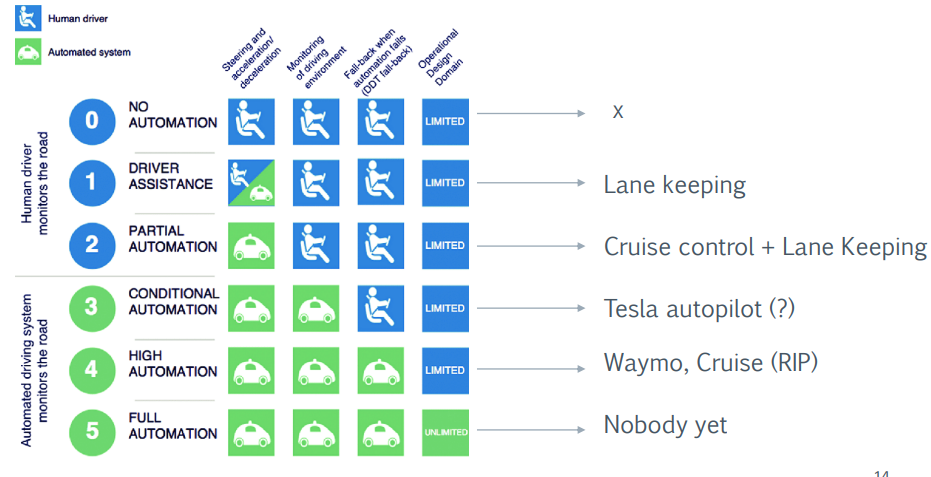
\includegraphics[width=0.5\textwidth]{images/C1_1.png}
    \label{fig:nome_immagine}
\end{wrapfigure}

But in \textbf{supervised driving} is the car operating autonomosly? today the SDC are mainly robotrucks or robotaxis, meanwhile any Teslea is not a true SDC.

SDC are robot that acts considering the \textbf{world model}, where the wolrd model is a probabilistc representation of the surronding enviroment, built from sensor data.
This is the really critical thing to do, modeling and interpreting the real world. Because:
\begin{compactitemize}
    \item Sensor provide \textbf{noisy, partial, and uncertain data}
    \item The vehivle must \textbf{predict and react intelligently} in an \textbf{unpredictable world}
\end{compactitemize}



\subsubsection{SAE Levels}

The Society of Automotive Engineers (SAE) defines different levels of driving automation according to the SAE J3016 standard. It provides a taxonomy with detailed definitions for six levels of driving automation, ranging from no driving automation (Level 0) to full driving automation (Level 5). The classification describes how driving tasks are progressively transferred from the human driver to the automated driving system.

The classification is based on three main aspects. It is all about:
\begin{compactitemize}
\item What the vehicle does;
\item Who supervises the driving;
\item Where the vehicle drives (ODD);
\item Who drives in the edges cases;
\end{compactitemize}

\subsubsection{Difference between ADAS and AD}
The principla differences are the folling ones:
\begin{compactitemize}
    \item Level of \textbf{control}: ADAS \textbf{assist the driver} with specific tasks, while AD involves full vehicle control with minimal or no human intervention.
    \item Driver \textbf{involvement}: ADAS \textbf{requires active driver partecipation}; AD aims to minimize or eliminate driver involvement.
    \item Scope of \textbf{functionality}: ADAS is focuses on enhancning safety and convenience in specific scenarios, while AD seeks to perform all driving tasks under various conditions.
    \item Technology and \textbf{complexity}: ADAS uses simpler algorithms and sensor setups compared to the more comples and integrated systems in AD.
\end{compactitemize}

\subsection{Thypes of AD}
There are three different type of AD, that are:
\begin{compactitemize}
    \item \textbf{Geometrical approach} (learned in this course)
    \item \textbf{End-to-End approach} (deel learning)
    \item \textbf{LLM-based approach} (Large Language Models and Multi-Modal AI)
\end{compactitemize}

\subsubsection{Geometrical approach}
In this approach, we use traditional computer vision, sensor fusion (LiDAR, radar), and rule-based algorithms for explicit geometric representations.

The principal \textbf{advantages} are that this technique allows us to have clear decision-making, reliability in structured environments, and is well-suited for known-knowns.

The main \textbf{challenges} are that it struggles with unstructured scenarios, has high computational demands, and has limited adaptability.
\begin{figure}[htbp]
    \centering
    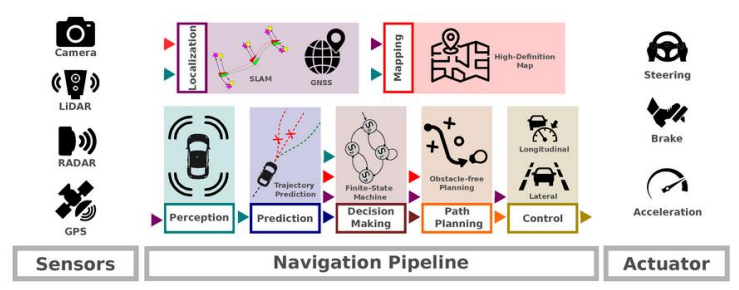
\includegraphics[width=0.65\textwidth]{images/C1_2.png}
    \label{fig:example}
\end{figure}

\paragraph{Sensor}
Different sensor are used for creating ADAs and AD applications:
\begin{compactitemize}
    \item \textbf{Camera}: is an electrinic device that sues lenses to capture images. It is used to detect and track objects or detect lane boundaries.
    \item \textbf{Radar}: is a technology system that uses radio waves to detect objects, their \textbf{distance, angle and speed} in relation to the ego-vehicle.
    \item \textbf{Lidar}: Light Detection and Ranging is a techonology used to scan objects, measure distances and height. A lidar sensore transmits laser beams that bounce off objects and return to the sensor.
    \item \textbf{GPS}: is a satellite-bases radio navigation which is used to provide a position, the GPS satellites broadcast two pieces of information: their \textbf{location} and  \textbf{time}.
\end{compactitemize}

\begin{infobox}[Sensor War]
There is an ongoing debate between LiDAR and cameras as the primary sensing technologies for autonomous vehicles. Tesla, as well as some systems associated with Mobileye, mainly rely on cameras combined with radar, while many other companies adopt a full sensor stack that includes LiDAR, cameras, radar, and other sensors. Tesla's approach is strongly associated with Elon Musk's criticism of LiDAR, which he considers expensive and unnecessary. He has argued that autonomous driving should be achievable using vision-based systems, pointing out that humans can drive without using LiDAR-like sensors. This difference in sensor strategies represents one of the main technological debates in autonomous driving.
\end{infobox}


\paragraph{Software stack}

\begin{wrapfigure}{r}{0.42\textwidth}
    \centering
    \vspace{-10pt}
    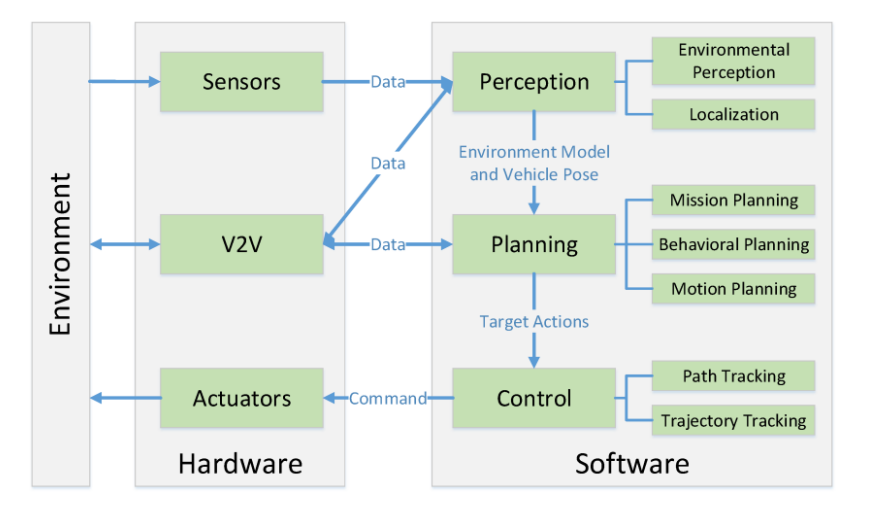
\includegraphics[width=\linewidth]{images/C1_3.png}
    \label{fig:new}
    \vspace{-10pt}
\end{wrapfigure}
The brain of the car is composed by three main components, that are:

\begin{compactitemize}
    \item \textbf{Perception}: This layer involves the detction and interpretation of the vehicle's surroundings using sensor like cameras, LIDAR and radar to identify objects.
    \item \textbf{Planning}: The decisio-making layer that determinates the vehicle's path and actions based on perceived data, considering route planning, obstacle avoidance, and maneuver exectuion.
    \item \textbf{Control}: This component manages the execution of planned actions by controlling the vehiclw's acceleration,braking, and steering to follow the desired path accurately and safely.
\end{compactitemize}

\paragraph{Perception}
The first thing that we do with the perception is the \textbf{enviromental perception} in which exxdntially extract meaninful information usign the aviabile sensor (typically camereas are the most used, but also LIDAR and ladar can be used).
The enviromental perception include also the \textbf{object detection} of the \textbf{dynamic object} like pedestrians or other vehicles and the \textbf{static objetcs} lije traffic light, sign ,ecc.

Other important thing that we can do using the perception is the \textbf{localization} that is the capacity of the camera to determiinate it's position in the world with low error, to do that we can use sensore like INS (GPS+IMU), LIDAR SLAM, Visual SLAM and fusion methods.

\paragraph{Sensor Fusion}
To overcome the limitations of the sensor, sensor fusion can be applied.
The sensor fusion provide redundancy for self-driving vehicles. For instance, LIDAR and Radare data can be fused to obtain an improved 3D object dectection independently of the weather contditons.

We'll use sensor fusion (radar+lidar) to improve the localization system of the car.

\paragraph{Path Planning}
\begin{wrapfigure}{R}{0.31\textwidth}
    \centering
    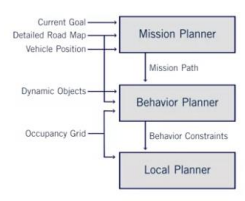
\includegraphics[width=0.3\textwidth]{images/C1_4.png}
    \label{fig:nome_immagine}
\end{wrapfigure}
Path planning is computational problem to find sequence of valid configurations or paths that moves the ego-vehicle from the source to destination.
There are three type of planning:
\begin{compactitemize}
    \item \textbf{Mission/global planning}: is the process of making the highes-level decision with regard to the proposed destination, for istance, which road should we take if we would like to go from Modena to Bologna.
    \item \textbf{Behavioral planning}: responsible for decision making to ensure the vehicle follows any stipulated road rules and interacts with other agents in a safe manner.
    \item \textbf{Motion/Local planning}: process of deciding on a sequence of action to reach a specified goal, typically while avoiding collision with obstacles (it defines the specific plan to drive).
\end{compactitemize}

\paragraph{Control}
The control computes and sends commands to the actuators of the steering wheel, threottle and brakes.

There are two type of control:
\begin{compactitemize}
    \item \textbf{Path tracking}: plan to move from start pose to a goal pose (\textbf{pure pursuit})
    \item \textbf{Trajectory tracking}: plan to move from a start pose to a goal includes the velocity (and time) information of the motion (\textbf{MPC}).
\end{compactitemize}

The controllers typically separates the problem in longitudinal and lateral control:
\begin{compactitemize}
    \item \textbf{Lateral control}: sterring angle.
    \item \textbf{Longitudianl control}: throttle and braking.
\end{compactitemize}

\paragraph{Remote driving}
Apart the pure AD there is also the remote driving that in the case of AD can be used to control the car when something goes wrong.

There are two type of remote control software:
\begin{compactitemize}
    \item \textbf{Operator SW}: software that process the infromation coming from the sensor (normally downsampled).
    \item \textbf{Operator to car SW}: control algorithms that process the commands from the operator (steering, brake, accelerator).
           The command can be \textbf{low level}, \textbf{medium level} (when the operator define a trajectory and shares the steer with the self drivinf sw) and \textbf{high level} command such as stop, go straight, etc.
\end{compactitemize}

\begin{figure}[htbp]
    \centering
    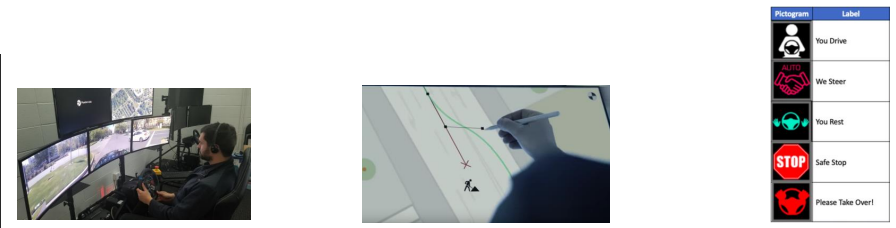
\includegraphics[width=0.8\textwidth]{images/C1_5.png}
    \caption{Low,medium and high level of remote commands}
\end{figure}

Remote driving technologies for self-driving cars typically involves a combination of various technologies to enable remote control and monitoring of the vehicles.

The principal technologies are:
\begin{compactitemize}
    \item \textbf{Teleoperation}: allow human operator remotely control a car. The operator can use a variety of input devices, such as joystick, steering wheels, or eventual reality interfaces.
    \item \textbf{High-speed data networks}: technology used to comunicate the information between the vehicle and operator.
    \item \textbf{Cameras and sensor}: the self-driving cars is equipped with multiple sensor to provide a comprehensive view of the vehicle's surroundings.
    \item \textbf{Remote control software}: the brain of the technology. Includes the sw that process the information coming from the sensor and the control algorithms that process the command from the operator.
\end{compactitemize}

\subsubsection{End-to-End autonomous driving}
Essentialy in this method we map sensor inputs directly to actions using deep neural networks, learning from large dataset.

The principal \textbf{advantages} are  that simply the pipeline, \textbf{learns complex patterns} and handle diverse conditions efficently.

The main \textbf{challenges} instead are that operates as a black box, depends heavilt on training data and strauggles with rare scenarios.

As you can see in the image below there are two type of end-to-end approach: the \textbf{full end-to-end}, and the \textbf{hybrid end-to-end}.
The principal difference between this two method is that in the full one the network take as input the raw sensor data anf return directly the action.
Instead in the hybrid we have the net do only same of the task of the original pipeline, for example it could create the trajectory but then is the mpc that choose the actions to take to follow the trajectory.

\begin{figure}[htbp]
    \centering
    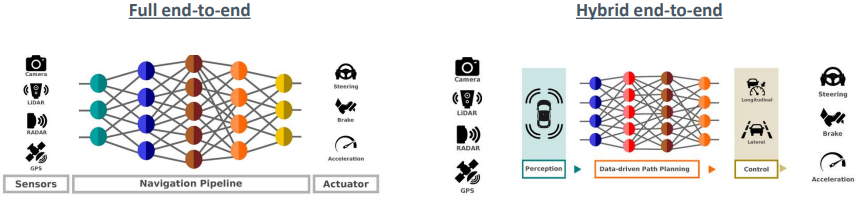
\includegraphics[width=0.9\textwidth]{images/C1_6.png}
    \caption{Low,medium and high level of remote commands}
\end{figure}

\subsubsection{LLM-based autonomous driving}
This method uses LLMs and multi-modal AI to assist in decison making, scenario interpretation, and human interaction.

The principal \textbf{advatnages} are that it's able to handle vast and dynamic scenarios, supports natural language inputs and adaptive learning.

The main \textbf{challenges} are the operates as a black box, has high computational need and has potential biases in decison-making.